\section{Reproducible illustrative results}
\label{sec:examples}
\newcommand{\BestOrder}{BAC}
\newcommand{\BestLoss}{11.00}

All quantities in this section are synthetic or analytically specified. They are not observations from the story, estimates from participants, or effects of an intervention. The accompanying Python program uses exact rational arithmetic for the scoring identity and enumerates every order and scenario in the scheduling example. Its JSON output and generated table are included in the project.

\subsection{A fragile efficient candidate and a robust alternative}
Consider two abstract candidate corridors with normalized nominal costs 1.00 and 1.25, clearances $c_A=0.12$ and $c_B=0.35$, and constraints $g_r=c_r-\delta$ for $|\delta|\leq\epsilon$. The scalar disturbance has sensitivity $L=1$. At $\epsilon=0.20$, their worst-case residuals are $-0.08$ and $0.15$. Thus A is nominally feasible and cheaper but fails under the permitted disturbance $\delta=0.20$; B remains feasible. Because the constraint is exactly affine, the worst-case residual here is exact. For general nonlinear problems a failed sufficient certificate does not itself prove infeasibility.

The cost and clearance values are assigned to make the tradeoff inspectable. They are not path lengths inferred from a physical geometry. No assertion is made about navigation engines, spacetime metrics, or real transport safety. Figure~\ref{fig:toys} shows where the margin vanishes as the disturbance bound increases.

\begin{figure}[htbp]
\centering
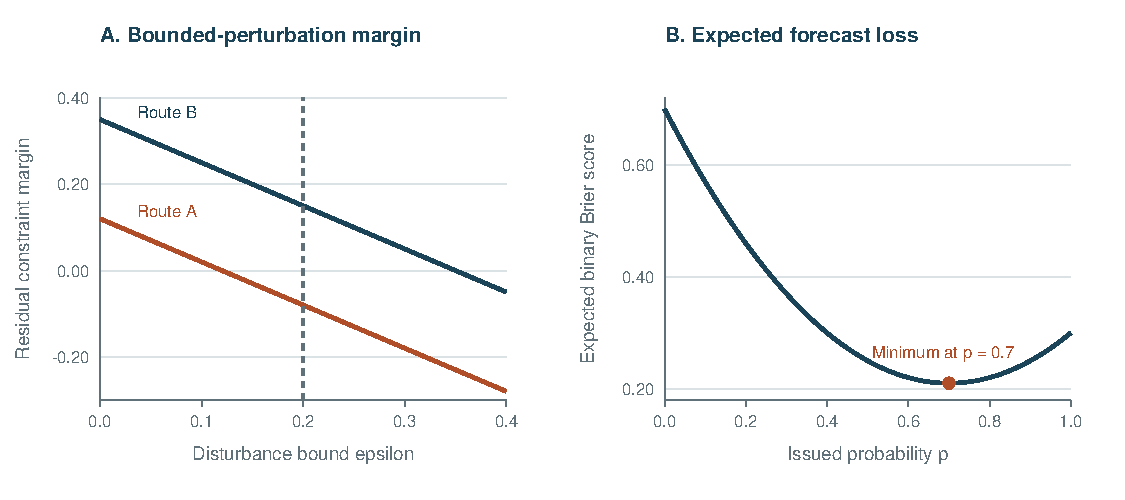
\includegraphics[width=\linewidth]{figures/toy_results.pdf}
\caption{Two deterministic mathematical illustrations. (A) Exact residual margins $c_r-\epsilon$ for abstract corridors; the dashed line marks $\epsilon=0.20$. (B) Expected binary Brier score for a Bernoulli event with $q=0.70$. The plotted curves are calculations, not fitted data.}
\label{fig:toys}
\end{figure}

\subsection{Confidence can increase expected loss}
With true event probability $q=0.70$, forecasts $p=0.50$, $0.70$, and $0.95$ have expected Brier scores $0.2500$, $0.2100$, and $0.2725$, respectively. Moving from a calibrated forecast to an overconfident one increases expected loss despite sounding more decisive. These are expectations under a known toy distribution, not a study showing that a particular training method improves confidence or accuracy.

\subsection{Allocation under uncertain loading}
Three jobs A, B, and C share one nonpreemptive server and are available at time zero. Loading times are independently $S_A\in\{1,5\}$ and $S_C\in\{2,4\}$, each with equal probability; $S_B=2$. Connection deadlines are $(4,3,7)$, delay weights $(1,2,1)$, and miss penalties $(10,8,6)$. For completion time $F_i$, define tardiness $D_i=\max(0,F_i-d_i)$ and a miss when $F_i>d_i$. Finishing exactly at the deadline is not a miss. The server follows a static permutation without idling and without knowing the future loading realizations.

\begin{table}[htbp]\centering\small
\begin{tabular}{lrrr}\toprule
Order & Expected loss & Expected tardiness & Expected misses\\\midrule
BAC & 11.00 & 3.00 & 1.00\\
BCA & 14.00 & 4.00 & 1.00\\
ABC & 18.00 & 4.00 & 1.50\\
ACB & 25.50 & 6.00 & 1.75\\
CBA & 26.00 & 6.00 & 2.00\\
CAB & 27.75 & 7.25 & 1.75\\
\bottomrule\end{tabular}
\caption{Exact enumeration for the four equally likely synthetic loading scenarios. Tardiness is summed across jobs in time units. The loss includes declared priority weights and missed-connection penalties.}\label{tab:schedules}
\end{table}

The best of the six enumerated static orders is \BestOrder{} with expected loss \BestLoss. For BAC the four scenario losses are $0,0,21,23$, whose mean is 11.00. This confirms only optimality within this finite policy class and these four equiprobable scenarios. An adaptive network policy has a different decision space. Changing priorities, deadlines, correlations, or available capacity can change the ranking. No confidential real routes were used, and this calculation supplies no privacy guarantee.

\subsection{The all-or-none bottleneck}
For thirty independent learners with identical success probability, $p^{30}$ is approximately 0.0424 for $p=0.90$, 0.2146 for $p=0.95$, and 0.7397 for $p=0.99$. These values demonstrate sensitivity of a collective endpoint to individual probabilities. They do not estimate any real graduation rate. Peer learning, shared instruction, and group stress can introduce dependence, so both benefit and harm must be evaluated rather than inferred from the formula.

\section{Prospective research protocols}
\label{sec:protocols}
The following are protocol proposals, not registered or completed studies. No sample size, approval, recruitment, clinical benefit, or successful intervention is claimed. Before data collection, freeze hypotheses, randomization, exclusion rules, primary outcomes, analysis code, and a power calculation based on a defensible minimally relevant effect. Simulation should assess the proposed estimator under missingness, realistic clustering, and uncertainty in effect size. A feasibility pilot should inform procedures without being relabeled as a confirmatory trial.

\subsection{Study A: robustness and scheduling benchmarks}
\textbf{Question.} Does a robust policy reduce constraint violations under disturbances represented in its uncertainty set, and at what cost? Compare a nominal optimizer, a robust optimizer, and a simple conservative baseline on released synthetic instances. Vary perturbation magnitude, model misspecification, network congestion, and available information. Freeze scenario generators and test sets separately from algorithm tuning.

\textbf{Outcomes and falsifiers.} Report violation rates with uncertainty, worst observed violation, nominal cost, compute time, missed connections, and unweighted and class-specific delays. An in-set violation despite a valid certificate would expose an implementation error, invalid bound, or violated assumption. Out-of-set failures characterize robustness limits. Report infeasibility explicitly rather than silently dropping difficult instances. Any separate privacy claim requires its own adjacency relation, leakage definition, composition analysis, and proof or adversarial evaluation.

\subsection{Study B: prediction-first physiological calibration}
\textbf{Design.} Randomly assign consenting adults to structured estimate--feedback training or a matched educational control with delayed aggregate feedback. Keep a blinded reference sensor recording in both groups. Predefine posture, estimation windows, rest intervals, display visibility, signal-quality exclusions, and the separate tasks for pulse and respiration. Collect confidence before revealing feedback and record participants' estimation strategies. Include an unfamiliar assessment context and a delayed retention visit.

\textbf{Primary estimand.} The difference between groups in change in held-out heart-rate MAE relative to a specified reference method. Respiration error, signed bias, interval coverage, confidence--accuracy association, and distress are secondary. Use a baseline-adjusted participant-level model or a prespecified hierarchical model; repeated trials are not independent participants. Analyze all randomized participants according to assignment, describe missingness, and perform stated sensitivity analyses. A practically null or adverse effect on the primary outcome would count against the training hypothesis even if self-reported confidence improved.

\textbf{Interpretation.} Performance relative to one device does not establish perfect awareness of internal physiology. Heartbeat counting is not the sole endpoint. The trial would not justify removing medically necessary monitoring or assuming that skill transfers to untested bodily variables.

\subsection{Study C: component testing of embodied updating}
\textbf{Design.} An eight-arm, parallel $2\times2\times2$ factorial study can compare (i) the source-inspired tapping locations versus matched alternative-location touch, (ii) comfortable paced breathing versus a matched period of unpaced breathing, and (iii) an evidence-revision cue versus neutral wording. Session duration, facilitator contact, task instructions, and expected plausibility should be matched as far as possible. Record expectancy and adherence. Participants cannot be fully blinded to action differences; analysts and outcome assessors can be masked to assignment.

\textbf{Task and primary outcome.} Use repeated probabilistic inference tasks with a declared generative model, new evidence, and later binary outcomes. Obtain forecasts before and after evidence, separating any bodily-state change from the factual revision. The primary outcome is mean post-evidence Brier score on held-out tasks, adjusted for baseline performance. Prespecify the main contrast for each factor and adjust for the three confirmatory comparisons; interactions and affective outcomes can be designated secondary unless the study is powered for them. A hierarchical model should account for participant and task dependence.

\textbf{Mechanistic limits.} This design tests tapping-location specificity, breath-pacing contribution, and cue contribution within a matched procedure. It does not isolate every ingredient, establish a meridian mechanism, or directly compare the whole package with no intervention. A separate no-touch control would be needed to estimate the contribution of rhythmic touch itself. Better mood without better inference would support an affective outcome only. More revision when evidence is uninformative could be a harmful increase in suggestibility. Report unchanged and worsening outcomes as well as improvements.

\subsection{Study D: cooperative learning without coercive certification}
\textbf{Design.} Randomize multiple intact learning groups to structured peer support with a collective milestone or to an equally resourced individual-progression program. Preserve individual certification and withdrawal in both arms. This intentionally tests a less coercive implementation of the source's cooperative idea; it is not a literal test of withholding every learner's credential until all pass.

\textbf{Outcomes.} The primary outcome is independently assessed individual mastery on unfamiliar tasks at a fixed follow-up. Secondary outcomes include delayed retention, dispersion of learning gains, time to mastery, helping behavior, assessment integrity, distress, exclusion, and perceived pressure. Assessors should be blind to group assignment. The group is the randomization unit; power and uncertainty must reflect the number of groups and intracluster correlation, not merely the number of learners. A single thirty-person cohort cannot identify the program's causal effect.

\subsection{Consent, data governance, and stopping rules}
Any human study requires prospective review by the responsible ethics body, individual informed consent, a clear withdrawal procedure, and avoidance of academic or interpersonal penalties for declining. Physiological recordings and personal inferences are sensitive data: collect the minimum necessary, separate identities from analysis records, define retention and access, and publish only appropriately governed outputs. The source's paired consent scene does not substitute for these procedures.

Breathing and attention tasks should permit ordinary comfortable breathing, immediate cessation for discomfort, and a prespecified response to adverse events. The proposed study need not use breath holds, hyperventilation, forced disclosure, sleep deprivation, or physical threat. Those would introduce additional interventions and risks unrelated to the central hypotheses. A stopping plan should specify who reviews adverse events and when recruitment or a procedure is suspended. These are research-design requirements, not claims that the narrative's practice is safe or unsafe in every setting.
